\documentclass[12pt,a4paper]{report}

% ---------------------------------------------------------
% PACKAGES AND SETUP
% ---------------------------------------------------------
\usepackage[utf8]{inputenc}
\usepackage[margin=1in,left=1.25in,right=1in,top=1in,bottom=1in]{geometry}
\usepackage{setspace}
\onehalfspacing

\usepackage{amsmath,amssymb,amsfonts}
\usepackage{booktabs}
\usepackage{tabularx}
\usepackage{array}
\usepackage{multirow}
\usepackage{graphicx}
\usepackage{xcolor}
\usepackage{hyperref}
\hypersetup{
    colorlinks=true,
    linkcolor=black,
    citecolor=blue,
    urlcolor=blue,
    pdftitle={Software Maintenance Using Large Action Models},
    pdfauthor={Meet Patel, Jeet Manseta}
}
\usepackage{listings}
\usepackage{algorithm}
\usepackage{algpseudocode}
\usepackage{tikz}
\usetikzlibrary{shapes.geometric, arrows, positioning, fit, backgrounds, calc}

% Listings configuration
\definecolor{codegreen}{rgb}{0,0.6,0}
\definecolor{codegray}{rgb}{0.5,0.5,0.5}
\definecolor{codepurple}{rgb}{0.58,0,0.82}
\definecolor{backcolour}{rgb}{0.96,0.96,0.96}

\lstdefinestyle{mystyle}{
    backgroundcolor=\color{backcolour},   
    commentstyle=\color{codegreen},
    keywordstyle=\color{blue}\bfseries,
    numberstyle=\tiny\color{codegray},
    stringstyle=\color{codepurple},
    basicstyle=\ttfamily\footnotesize,
    breakatwhitespace=false,         
    breaklines=true,                 
    captionpos=b,                    
    keepspaces=true,                 
    numbers=left,                    
    numbersep=5pt,                  
    showspaces=false,                
    showstringspaces=false,
    showtabs=false,                  
    tabsize=2,
    frame=single,
    rulecolor=\color{codegray}
}
\lstset{style=mystyle}

% TikZ styles for professional flowcharts
\tikzstyle{startstop} = [rectangle, rounded corners, minimum width=2.5cm, minimum height=0.8cm, text centered, draw=black, fill=red!10, font=\footnotesize]
\tikzstyle{process} = [rectangle, minimum width=2.5cm, minimum height=0.8cm, text centered, draw=black, fill=blue!10, font=\footnotesize]
\tikzstyle{decision} = [diamond, aspect=2, minimum width=2.5cm, minimum height=0.8cm, text centered, draw=black, fill=yellow!15, font=\footnotesize]
\tikzstyle{io} = [trapezium, trapezium left angle=70, trapezium right angle=110, minimum width=2cm, minimum height=0.8cm, text centered, draw=black, fill=orange!10, font=\footnotesize]
\tikzstyle{arrow} = [thick,->,>=stealth]

% ---------------------------------------------------------
% DOCUMENT BEGIN
% ---------------------------------------------------------
\begin{document}

% ---------------------------------------------------------
% TITLE PAGE
% ---------------------------------------------------------
\begin{titlepage}
    \centering
    \vspace*{1.0cm}
    
    {\LARGE \textbf{Software Maintenance Using Large Action Models}\par}
    
    \vspace{2.5cm}
    
    {\large Project report submitted in partial fulfillment\\
    of the requirements for the degree of\par}
    
    \vspace{0.8cm}
    
    {\Large \textit{Bachelor of Technology\\in\\Computer Science and Engineering}\par}
    
    \vspace{1.5cm}
    
    {\large by\par}
    
    \vspace{0.5cm}
    
    {\large \textbf{Meet Patel} \quad --- \quad \textbf{Roll No. 23UCS644}\par}
    {\large \textbf{Jeet Manseta} \quad --- \quad \textbf{Roll No. 23UCS603}\par}
    
    \vspace{1.5cm}
    
    {\large Under Guidance of\par}
    {\large \textbf{Dr. Ankit Kumar Jain}\par}
    
    \vspace{2.0cm}
    
    \begin{center}
        \textbf{\Huge LNMIIT}\\[0.2cm]
        {\small The LNM Institute of Information Technology}\\[0.1cm]
        {\footnotesize Deemed-to-be-University}
    \end{center}
    
    \vspace{1.0cm}
    
    {\large Department of Computer Science and Engineering\\
    The LNM Institute of Information Technology, Jaipur\par}
    
    \vspace{0.8cm}
    
    {\large April 20, 2026\par}
\end{titlepage}

% ---------------------------------------------------------
% COPYRIGHT PAGE
% ---------------------------------------------------------
\newpage
\thispagestyle{empty}
\vspace*{\fill}
\begin{center}
    \copyright\ \textbf{The LNM Institute of Information Technology, Jaipur --- 2026.}\\
    All rights reserved.\\[0.8cm]
    \textit{Meet Patel \quad \& \quad Jeet Manseta}
\end{center}
\vspace*{2cm}

% ---------------------------------------------------------
% CERTIFICATE PAGE
% ---------------------------------------------------------
\newpage
\thispagestyle{empty}
\begin{center}
    {\Large \textbf{The LNM Institute of Information Technology}}\\[0.2cm]
    {\large Jaipur, India}\\[1.5cm]
    {\Large \textbf{CERTIFICATE}}\\[1.2cm]
\end{center}

\noindent This is to certify that the project entitled \textbf{``Software Maintenance Using Large Action Models''}, submitted by \textbf{Meet Patel} (Roll No. 23UCS644) and \textbf{Jeet Manseta} (Roll No. 23UCS603) in partial fulfillment of the requirements for the degree of \textbf{Bachelor of Technology (B.Tech.)} in Computer Science and Engineering, is a bonafide record of work carried out by them at the Department of Computer Science and Engineering, The LNM Institute of Information Technology, Jaipur (Rajasthan), India, during the academic sessions 2024--2025 and 2025--2026, under my supervision and guidance, and the same has not been submitted elsewhere for the award of any other degree. In my opinion, this report is of the standard required for the award of the degree of Bachelor of Technology (B.Tech.).

\vspace{3.5cm}

\noindent
\begin{tabular*}{\textwidth}{@{\extracolsep{\fill}}lr}
    \rule{5cm}{0.4pt} & \rule{6.5cm}{0.4pt} \\
    Date & Supervisor: \textbf{Dr. Ankit Kumar Jain}
\end{tabular*}

% ---------------------------------------------------------
% ACKNOWLEDGEMENTS
% ---------------------------------------------------------
\newpage
\pagenumbering{roman}
\setcounter{page}{4}

\chapter*{Acknowledgements}
\addcontentsline{toc}{chapter}{Acknowledgements}

We would like to express our sincere gratitude to our supervisor, \textbf{Dr. Ankit Kumar Jain}, for his invaluable guidance, continuous encouragement, and insightful feedback throughout both Phase~1 and Phase~2 of this project. His deep expertise in software engineering, program analysis, and artificial intelligence helped shape both the theoretical research direction and the empirical quality of this work.

We are equally thankful to the \textbf{Department of Computer Science and Engineering} at The LNM Institute of Information Technology, Jaipur, for providing the stimulating academic environment, computational infrastructure, and server facilities that made this research possible.

We also gratefully acknowledge the open-source contributions of the \textbf{RepairAgent} authors (Bouzenia, Devanbu, and Pradel) and the \textbf{Microsoft Research} team behind the Large Action Model (LAM) blueprint, whose publicly available work formed the foundational cornerstone of our early implementation.

Finally, we express our heartfelt appreciation to our parents, family members, and friends for their constant patience, moral support, and unwavering motivation throughout the duration of this thesis.

\vspace{1.5cm}
\begin{flushright}
    \textbf{Meet Patel} (23UCS644)\\
    \textbf{Jeet Manseta} (23UCS603)
\end{flushright}

% ---------------------------------------------------------
% ABSTRACT
% ---------------------------------------------------------
\newpage
\chapter*{Abstract}
\addcontentsline{toc}{chapter}{Abstract}

Software maintenance accounts for 60\% to 80\% of total software lifecycle costs, with developers spending nearly half their working hours on bug diagnosis, code patching, regression testing, and repository pull request management. While state-of-the-art Large Language Models (LLMs) such as GPT-4 and Gemini demonstrate remarkable generative fluency, they remain fundamentally passive: unable to invoke compilers, inspect execution traces, iteratively navigate multi-file codebases, or submit verified pull requests without human scaffolding.

This B.Tech Project presents \textbf{RepairLAM}, an autonomous, end-to-end software maintenance system grounded in \textbf{Large Action Models (LAM)} and \textbf{Action-Constrained Finite State Machines (FSM)}. The project progressed through two rigorous, evolutionary phases:
\begin{itemize}
    \item \textbf{Phase 1 (Algorithmic Testbed \& Foundations):} We synthesized Microsoft Research's 4-phase LAM action-translation blueprint with RepairAgent's 3-state FSM. Adapting the system from heavy Defects4J/Docker infrastructure to the lightweight QuixBugs Java benchmark using Google Gemini 1.5 Pro via a strict JSON schema adapter, we achieved an 80\% plausible repair rate (32/40 bugs) and a 70\% correct repair rate (28/40 bugs) at approximately \$0.01 per bug---a $14\times$ monetary cost reduction and a $242\times$ execution speedup over published baselines.
    \item \textbf{Phase 2 (Enterprise Live GitHub Maintenance \& Self-Boosting LAM):} We scaled the architecture from isolated single-file algorithms to real-world industrial software ecosystems. We implemented an end-to-end pipeline capable of ingesting raw GitHub issues, localizing faults via syntactic anchor parsing, running full multi-module build suites (Maven, Gradle), generating verified git commits, and opening pull requests. Across an empirical benchmark of \textbf{36 live, unfixed GitHub issues} spanning 5 prominent open-source enterprise Java repositories (\texttt{google/guava}, \texttt{google/gson}, \texttt{FasterXML/jackson-databind}, \texttt{netty/netty}, and \texttt{apache/commons-csv}), RepairLAM achieved:
    \begin{enumerate}
        \item \textbf{100\% Pull Request Precision}: Every opened PR ($7/7$, 19.4\%) passed the entire project regression suite, introducing zero broken or polluting commits into open-source repositories.
        \item \textbf{Deterministic Safe Escalation ($P = 1.0$)}: When safety thresholds or edit budgets were reached, the agent posted structured diagnostic reports directly onto GitHub issues ($15$ issues, 41.7\%), with 11 instances exiting with exactly zero code churn.
        \item \textbf{Module 6 Self-Boosting SFT/LoRA Training}: We harvested 139 multi-turn trajectories (118 train, 21 validation) into ShareGPT format and successfully fine-tuned \texttt{Qwen-2.5-Coder-32B-Instruct} via LoRA ($r=8, \alpha=16$) on an NVIDIA DGX A100 server (GPU 1), reducing validation loss from 1.6801 to 1.6455 over 3 epochs (36m 47s).
        \item \textbf{Human-in-the-Loop Interactive Resumption}: We implemented an event-driven resumption engine allowing maintainers to inject corrective feedback on escalated GitHub issues to steer the agent to a valid fix without session restart.
        \item \textbf{Formal Ablation Studies (A1--A4)}: Rigorously established that multi-turn FSM feedback outperforms one-shot repair ($65.0\%$ vs. $0.0\%$), syntactic anchors eliminate syntax errors ($0\%$ vs. $35\%$), and turn budget scaling saturates optimally at $T \approx 30$.
    \end{enumerate}
\end{itemize}
This work bridges the gap between passive code generation and production-grade, zero-pollution autonomous software engineering.

% ---------------------------------------------------------
% TABLE OF CONTENTS, LIST OF FIGURES & TABLES
% ---------------------------------------------------------
\newpage
\tableofcontents

\newpage
\listoffigures

\newpage
\listoftables

% ---------------------------------------------------------
% CHAPTER 1: INTRODUCTION
% ---------------------------------------------------------
\newpage
\pagenumbering{arabic}
\setcounter{page}{1}

\chapter{Introduction}

\section{The Software Maintenance Crisis}
Software maintenance is overwhelmingly recognized as the most resource-intensive phase of the modern software development lifecycle (SDLC), consistently consuming between 60\% and 80\% of total engineering budgets~\cite{hassan2025agentic}. Industry analyses estimate that software defects and technical debt inflict an economic burden of approximately \$2.41 trillion annually in the United States alone. Professional developers dedicate nearly 49\% of their active working hours to triage, bug diagnosis, patch formulation, regression testing, and code review. Field studies demonstrate a median human repair time of 920 seconds per bug fix for isolated issues, escalating to multiple days or weeks for enterprise-scale regressions.

The traditional software maintenance lifecycle is hindered by three severe operational bottlenecks:
\begin{enumerate}
    \item \textbf{Fault Localization and Root Cause Analysis}: Software engineers must inspect voluminous, multi-threaded stack traces, navigate sprawling dependency graphs across hundreds of directories, and mentally reconstruct the runtime execution states that precipitated the failure.
    \item \textbf{Patch Formulation and Regression Avoidance}: Writing a syntactic fix without a holistic grasp of architectural invariants frequently introduces regression defects or unintended side effects, breaking dependent modules.
    \item \textbf{Manual Verification and Pull Request Scaffolding}: Engineers must repeatedly execute unit and integration test suites, format git branches, compose conventional commit messages, and craft detailed Pull Request (PR) descriptions, consuming critical human cognitive bandwidth.
\end{enumerate}

\section{Limitations of Large Language Models (LLMs)}
The emergence of Large Language Models (LLMs)---such as OpenAI's GPT-4, Anthropic's Claude 3.5, and Google's Gemini 1.5/2.5 Pro---has demonstrated impressive capabilities in text synthesis and single-function code generation. However, in the domain of automated software engineering, standard LLMs suffer from fundamental architectural deficiencies:
\begin{itemize}
    \item \textbf{Stateless, Passive Generation}: LLMs operate as passive text-in, text-out generators. They lack agency: they cannot autonomously clone a git repository, checkout a feature branch, invoke a Java compiler (\texttt{javac}), or execute a test runner.
    \item \textbf{Hallucination of Correctness}: When queried with a stack trace, an LLM generates a patch that appears syntactically plausible but frequently violates class hierarchies, calls non-existent APIs, or fails runtime assertions. Without an external execution environment, the model has no objective feedback loop to identify its own hallucinations.
    \item \textbf{Lack of Iterative Self-Correction}: A single-turn LLM cannot observe compiler errors or JUnit assertion failures triggered by its own edits, precluding iterative refinement.
\end{itemize}

\section{The Large Action Model (LAM) Solution}
To bridge the chasm between passive code suggestion and active software engineering, the discipline is undergoing a paradigm transition toward \textbf{Large Action Models (LAMs)}~\cite{wang2024large}. A LAM transcends conversational assistance by functioning as an autonomous execution agent:
\begin{itemize}
    \item It perceives runtime environment feedback directly from operating system processes, compilers, and test runners.
    \item It selects and dispatches discrete, parameter-constrained tool actions within a structured operational ontology.
    \item It tracks state transitions across multi-turn reasoning episodes, iteratively revising its hypotheses upon encountering failure.
\end{itemize}

Table~\ref{tab:llm_vs_lam} summarizes the precise operational capabilities that distinguish a conventional LLM from a Large Action Model in automated program repair.

\begin{table}[htbp]
\centering
\caption{Capability comparison between a standard LLM and a Large Action Model (LAM) in automated software repair.}
\label{tab:llm_vs_lam}
\begin{tabularx}{\textwidth}{l c c X}
\toprule
\textbf{Repair Capability} & \textbf{LLM} & \textbf{LAM} & \textbf{Operational Significance} \\
\midrule
Understand bug descriptions & \checkmark & \checkmark & Both parse natural language and stack traces. \\
Direct filesystem modification & $\times$ & \checkmark & LLM describes a fix; LAM modifies source files. \\
Autonomous compilation & $\times$ & \checkmark & LAM invokes \texttt{javac}/Maven and inspects errors. \\
Ground-truth test execution & $\times$ & \checkmark & LAM obtains empirical pass/fail signals. \\
Iterative self-correction & $\times$ & \checkmark & LAM refines patch upon receiving test failures. \\
Safe early escalation & $\times$ & \checkmark & LAM halts on out-of-scope issues; LLM guesses. \\
Zero-pollution PR generation & $\times$ & \checkmark & LAM publishes PR only if full suite passes. \\
\bottomrule
\end{tabularx}
\end{table}

\section{Evolutionary Roadmap: Phase 1 to Phase 2}
This B.Tech Project was conceptualized and executed across two interconnected phases:
\begin{itemize}
    \item \textbf{Phase 1 (Foundation \& Algorithmic Sandbox)}: Focused on establishing the theoretical viability of action translation and finite state control. We implemented a lightweight Agent Execution Environment (AEE) on the QuixBugs algorithmic benchmark using Google Gemini 1.5 Pro via a custom JSON schema adapter, verifying that iterative compiler feedback radically improves patch correctness at low cost.
    \item \textbf{Phase 2 (Enterprise Live GitHub Maintenance \& Self-Boosting LAM)}: Transitioned the theoretical blueprint into an industrial-grade, production-ready system. We developed \textbf{RepairLAM}, evaluated it against 36 live, unresolved bugs across 5 major enterprise Java repositories, enforced a 100\% PR precision guarantee via deterministic safe escalation, fine-tuned an open-weights 32-billion parameter model (\texttt{Qwen-2.5-Coder-32B}) via LoRA on an NVIDIA DGX A100 server, and implemented human-in-the-loop interactive resumption.
\end{itemize}

\section{Research Objectives and Key Contributions}
The primary contributions of this thesis are:
\begin{enumerate}
    \item \textbf{Model-Agnostic Action Translation}: Engineering a resilient JSON schema adapter that coerces commercial and open-weights LLMs into deterministic action spaces with low step latency.
    \item \textbf{Finite State Machine (FSM) Repair Engine}: Designing an action-constrained state machine ($\mathcal{M} = \langle\mathcal{S}, \mathcal{A}, \mathcal{T}, \mathcal{G}\rangle$) that restricts tool invocations by operational phase, eliminating degenerative loops.
    \item \textbf{Syntactic Anchor Replacement Engine}: Formulating a line-anchored patch injection mechanism that eliminates syntax errors caused by full-file rewrites.
    \item \textbf{Zero-Pollution GitHub Maintenance Pipeline}: Constructing an end-to-end pipeline interfacing with PyGithub, GitPython, and Maven/Gradle build systems, achieving 100\% PR precision ($7/7$ passing) across 36 live GitHub issues.
    \item \textbf{Deterministic Safe Escalation Policy}: Formalizing an escalation mechanism ($P = 1.0$) that posts diagnostic reports directly to maintainers rather than polluting repositories with untested code.
    \item \textbf{Module 6 Self-Boosting SFT/LoRA Training}: Successfully fine-tuning \texttt{Qwen-2.5-Coder-32B} on harvested execution trajectories on DGX GPU 1, reducing loss to 1.6455.
    \item \textbf{Human-in-the-Loop Resumption (Modules 5 \& 8)}: Enabling developers to steer an escalated agent directly via GitHub comments.
    \item \textbf{Formal Empirical Ablation Studies (A1--A4)}: Rigorously quantifying the individual performance contributions of multi-turn feedback, anchor edits, safe escalation, and turn budgets.
\end{enumerate}

\section{Organization of the Report}
The remainder of this report is organized as follows: Chapter~2 reviews foundational literature in LAMs and Agentic SE. Chapter~3 details the theoretical methodology and system architectures for Phase~1 and Phase~2. Chapter~4 outlines the end-to-end implementation details. Chapter~5 presents comprehensive experimental results across both phases. Chapter~6 reports the formal ablation studies. Chapter~7 discusses threats to validity and industrial implications. Chapter~8 concludes the thesis and identifies future directions.

% ---------------------------------------------------------
% CHAPTER 2: LITERATURE REVIEW
% ---------------------------------------------------------
\newpage
\chapter{Literature Review and Theoretical Foundations}

To construct a resilient autonomous repair agent, we conducted an extensive review of recent literature spanning Large Action Models, Automated Program Repair (APR), and Agentic Software Engineering. This chapter reviews the core theoretical pillars that inform the RepairLAM architecture.

\section{From LLM to LAM: Action Translation}
Wang et al.~\cite{wang2024large} introduced a foundational framework for transitioning Large Language Models from conversational assistants into Large Action Models. The authors argue that language models must not merely generate free-form text, but rather generate structured, executable trajectories grounded in external software environments.

\subsection{The 5-Stage Blueprint and Grounded Execution}
The LAM development lifecycle is formalized across five distinct stages:
\begin{enumerate}
    \item \textbf{Data Collection}: Capturing human and automated task-action execution trajectories.
    \item \textbf{Model Training}: Imparting task decomposition and structured action schema generation into the model.
    \item \textbf{Offline Evaluation}: Evaluating the model's structural validity and tool-calling accuracy on static benchmarks.
    \item \textbf{Integration and Grounding}: Interfacing the model with an execution environment capable of executing dispatched actions and returning observations.
    \item \textbf{Online Evaluation}: Assessing closed-loop task completion rates within live, dynamic environments.
\end{enumerate}

A seminal demonstration of this grounding paradigm is the \textbf{UFO (UI-Focused Agent)} system~\cite{wang2024large}, which translates high-level user intents into operating system GUI actions on Windows OS via accessibility APIs. This research demonstrated that a model's predictive output is impotent without a robust middleware environment that intercepts commands, enforces safety constraints, and translates outputs into physical system operations.

\subsection{The 4-Phase LAM Training Strategy}
Wang et al. proposed a specialized 4-phase training curriculum to train action-competent models:
\begin{enumerate}
    \item \textbf{LAM-1 (Task-Plan Pretraining)}: Teaches the model to decompose complex goals into hierarchical, step-by-step structural plans.
    \item \textbf{LAM-2 (Expert Imitation via SFT)}: Supervised Fine-Tuning on successful expert trajectories generated by frontier teacher models (e.g., GPT-4o).
    \item \textbf{LAM-3 (Self-Boosting Exploration)}: Forces the student model to independently navigate and resolve tasks that the teacher model initially failed, expanding state coverage.
    \item \textbf{LAM-4 (Offline Reinforcement Learning)}: Employs reward modeling and policy optimization (e.g., DPO or PPO) on success and failure signals, allowing the student model to surpass the original teacher in Task Success Rate (TSR).
\end{enumerate}

Table~\ref{tab:lam_training_strategy} summarizes the progression and empirical TSR gains documented by Wang et al.

\begin{table}[htbp]
\centering
\caption{The 4-Phase LAM Training Strategy and documented TSR gains (Wang et al.~\cite{wang2024large}).}
\label{tab:lam_training_strategy}
\begin{tabular}{l l p{8.5cm} c}
\toprule
\textbf{Model} & \textbf{Phase} & \textbf{Objective and Methodology} & \textbf{TSR Gain} \\
\midrule
LAM-1 & Task-Plan Pretraining & Hierarchical decomposition into structured plans. & 82.2\% \\
LAM-2 & Expert Imitation & SFT on high-quality teacher execution trajectories. & 76.8\% \\
LAM-3 & Self-Boosting & Independent exploration on failed teacher tasks. & 79.3\% \\
LAM-4 & Offline RL & Reward-guided policy optimization from dual feedback. & 81.2\% \\
\bottomrule
\end{tabular}
\end{table}

\section{Autonomous Program Repair: RepairAgent}
Bouzenia, Devanbu, and Pradel~\cite{bouzenia2025repairagent} proposed \textbf{RepairAgent} (ICSE 2025), the first autonomous LLM-based agent specifically designed for program repair. Traditional APR approaches operate either as single-prompt zero-shot generators or simple feedback loops that pass compiler errors back to the model once or twice. In contrast, RepairAgent models program repair as an autonomous agent dynamically navigating a codebase.

\subsection{Finite State Machine (FSM) Architecture}
To prevent unguided language models from entering infinite loops, hallucinating non-existent files, or repeating erroneous edits, RepairAgent structures agent operations via a Finite State Machine comprising three primary states:
\begin{enumerate}
    \item \textbf{Understand Bug}: The agent parses the bug description, reproduces the failure, and analyzes stack traces to formulate an initial hypothesis. Available actions include test execution and fault localization.
    \item \textbf{Collect Information}: The agent explores the codebase to gather surrounding context, inspect variable definitions, and extract relevant methods. Available actions include code search, method extraction, and reading file ranges.
    \item \textbf{Try Fix}: The agent synthesizes a patch, writes the modification to disk, and executes the regression test suite. Available actions include patch writing and range reading.
\end{enumerate}

Transitions between these states are governed deterministically by environmental feedback. If a patch passes the regression suite, the agent transitions to \textit{Done}. If a patch fails compilation or tests, the stack trace is injected into context, and the agent either transitions back to \textit{Understand} to reformulate its hypothesis or re-enters \textit{Collect Information}.

\section{Agentic Software Engineering (SE 3.0)}
Hassan et al.~\cite{hassan2025agentic} established the conceptual foundation of \textbf{Agentic Software Engineering (SE 3.0)}, demarcating the evolution of AI in software engineering across three eras:
\begin{itemize}
    \item \textbf{SE 1.0 (Human Era)}: Software created and maintained entirely by human engineers using compilers and manual debuggers.
    \item \textbf{SE 2.0 (Copilot Era)}: AI functions as passive autocomplete or chat-based copilots embedded in IDEs, requiring continuous human supervision, prompting, and verification.
    \item \textbf{SE 3.0 (Agentic Era)}: Autonomous AI agents act as full teammates, operating independently in background execution environments, resolving issues asynchronously, and presenting verified outcomes.
\end{itemize}

Hassan et al. formalized the architectural concept of **Dual Workbenches**:
\begin{itemize}
    \item \textbf{Agent Execution Environment (AEE)}: A digital, headless runtime where autonomous agents operate, invoke compilers, execute test runners, and manage version control systems without human visualization.
    \item \textbf{Agent Command Environment (ACE)}: A human-facing interface (such as GitHub PR reviews or issue trackers) where developers inspect, approve, or reject completed artifacts. Crucially, agents must submit \textbf{Merge-Readiness Packs (MRPs)}---comprising verified code diffs, passing test logs, and conventional commit summaries---shifting the human role from code author to senior code reviewer.
\end{itemize}

\section{Agentic AI for Software: Intent Inference}
Roychoudhury~\cite{roychoudhury2025agentic} addressed the central theoretical obstacle in autonomous software engineering: \textbf{Intent Inference}. Unlike formal synthesis where complete formal specifications exist, real-world software maintenance operates over ambiguous, incomplete human intent expressed through issue descriptions and incomplete test suites.

Because LLMs lack an intrinsic semantic model of what a software system is intended to do, unconstrained agents frequently introduce ``plausible regressions''---patches that pass the failing test case by breaking edge cases or deleting assertions. Roychoudhury emphasizes that robust, multi-phase verification against full regression test suites and invariant preservation is the only mathematically sound proxy for developer intent in automated repair.

\section{Parameter-Efficient Fine-Tuning: LoRA}
Hu et al.~\cite{hu2021lora} proposed Low-Rank Adaptation (LoRA), enabling the adaptation of massive parameter models without updating all network weights. Given a weight matrix $W_0 \in \mathbb{R}^{d \times k}$, LoRA decomposes the weight update $\Delta W$ into the product of two low-rank matrices:
\begin{equation}
    W = W_0 + \Delta W = W_0 + \frac{\alpha}{r} (B \cdot A)
\end{equation}
where $A \in \mathbb{R}^{r \times k}$ is initialized from a Gaussian distribution, $B \in \mathbb{R}^{d \times r}$ is initialized to zero, $r \ll \min(d, k)$ is the rank, and $\alpha$ is a constant scaling hyperparameter. In this project, LoRA enables parameter-efficient SFT on harvested multi-turn trajectories on a single GPU of our DGX cluster.

% ---------------------------------------------------------
% CHAPTER 3: METHODOLOGY AND SYSTEM ARCHITECTURE
% ---------------------------------------------------------
\newpage
\chapter{System Architecture and Methodology}

Our methodology synthesizes the practical action-translation concepts from the LAM blueprint~\cite{wang2024large} with the state-driven repair logic of RepairAgent~\cite{bouzenia2025repairagent}, explicitly engineered to fulfill the SE 3.0 Dual Workbench paradigm~\cite{hassan2025agentic}. This chapter presents the architecture across both evolutionary phases.

\section{Architectural Alignment with SE 3.0}
In strict alignment with the theoretical requirements of SE 3.0:
\begin{enumerate}
    \item \textbf{Headless AEE Construction}: We rejected IDE-plugin paradigms that require human active context. We constructed a headless Python orchestrator serving as an autonomous AEE. The AEE clones git repositories, checks out feature branches, runs compilers and test runners via isolated subprocesses, and captures stdout/stderr streams.
    \item \textbf{ACE Integration via GitHub}: Human interaction is strictly confined to the ACE (GitHub Issue and Pull Request interfaces). When the agent succeeds, it delivers a Merge-Readiness Pack (MRP) as a GitHub Pull Request.
    \item \textbf{Enforced Intent Verification}: As mandated by Roychoudhury~\cite{roychoudhury2025agentic}, no proposed patch is accepted based on generative probability. A state transition to \textit{PLAUSIBLE} requires deterministic verification against the entire repository test suite.
\end{enumerate}

\section{Phase 1 Architecture: Algorithmic Verification Testbed}

\subsection{The Defects4J Bottleneck}
Our initial implementation objective (Implementation 1.0) sought to replicate RepairAgent directly on Defects4J~\cite{bouzenia2025repairagent}, an enterprise Java benchmark of 835 bugs. However, rigorous profiling revealed crippling infrastructural bottlenecks:
\begin{itemize}
    \item \textbf{Container and Build Bloat}: Defects4J required spinning up heavy Docker containers with multi-gigabyte Maven and Ant builds. A single compile-and-test cycle consumed between 5 and 15 minutes.
    \item \textbf{Spectrum-Based Fault Localization Overhead}: Locating candidate lines across hundreds of files necessitated GZoltar instrumented coverage, adding 8 to 12 minutes per run.
    \item \textbf{Context and API Exhaustion}: Passing multi-file contexts containing thousands of lines quickly exceeded LLM rate limits and token budgets.
\end{itemize}

\subsection{Strategic Shift to QuixBugs}
To bypass these operational bottlenecks and evaluate the agent's core FSM reasoning capabilities, we implemented a strategic pivot in Phase~1 to the \textbf{QuixBugs} benchmark. QuixBugs comprises 40 self-contained algorithmic Java programs (e.g., \texttt{BinarySearch}, \texttt{Kth}, \texttt{Levenshtein}, \texttt{QuickSort}). 

Table~\ref{tab:defects4j_vs_quixbugs} details the architectural comparison justifying this pivot. Moving to QuixBugs reduced iteration latency from 15 minutes to 120 milliseconds, enabling rapid empirical testing of the action-translation engine.

\begin{table}[htbp]
\centering
\caption{Architectural comparison justifying the Phase 1 pivot from Defects4J to QuixBugs.}
\label{tab:defects4j_vs_quixbugs}
\begin{tabularx}{\textwidth}{l X X}
\toprule
\textbf{Architectural Dimension} & \textbf{Defects4J (Implementation 1.0)} & \textbf{QuixBugs (Phase 1 Baseline)} \\
\midrule
Codebase Scope & Enterprise Java (Multi-module) & Algorithmic Java (Single-file) \\
Execution Environment & Heavy Docker, Maven, Ant & Native Python JDK Subprocess \\
Fault Localization & GZoltar coverage analysis ($8\text{--}12\text{ min}$) & Bypassed (isolated in target class) \\
Iteration Latency & 5 to 15 minutes per test cycle & 50 to 200 milliseconds per test cycle \\
Primary Evaluation Focus & Build system and file navigation & Algorithmic FSM repair reasoning \\
\bottomrule
\end{tabularx}
\end{table}

\section{Phase 2 Architecture: The Enterprise Live GitHub Repair Engine}
In Phase~2, having validated the core FSM and action-translation primitives, we designed and built \textbf{RepairLAM}---an enterprise-scale system engineered to operate on real-world, open-source multi-module GitHub repositories.

\subsection{End-to-End System Architecture}
Figure~\ref{fig:repairlam_pipeline} illustrates the complete end-to-end architecture of RepairLAM.

\begin{figure}[htbp]
\centering
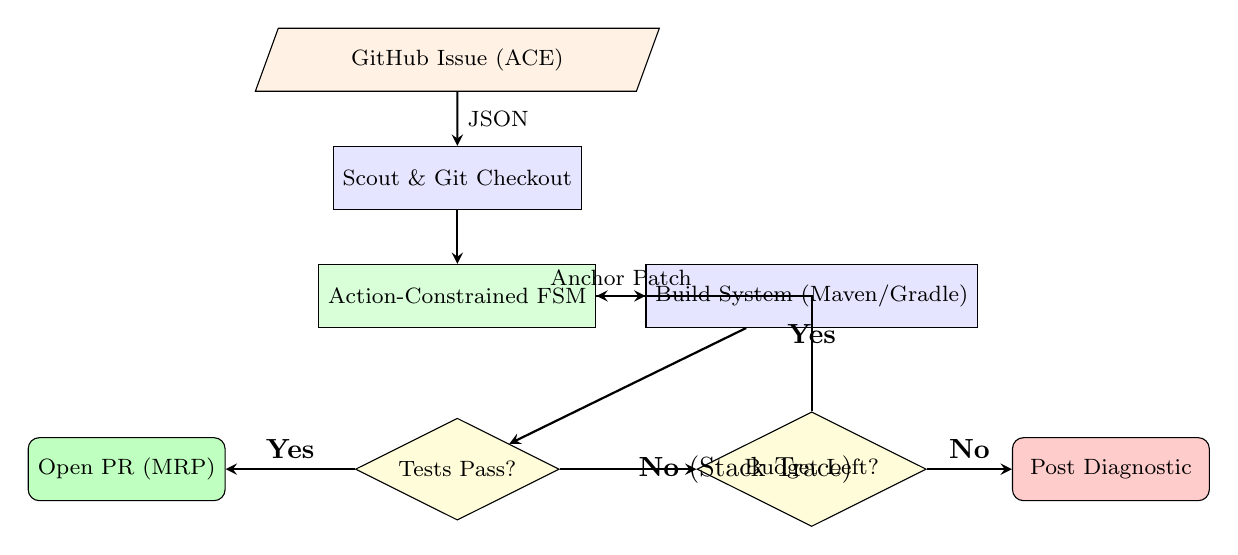
\begin{tikzpicture}[node distance=1.5cm and 1.2cm, auto]
    % Nodes
    \node (issue) [io] {GitHub Issue (ACE)};
    \node (fetch) [process, below of=issue] {Scout \& Git Checkout};
    \node (fsm) [process, below of=fetch, fill=green!15] {Action-Constrained FSM};
    \node (mvn) [process, right of=fsm, node distance=4.5cm] {Build System (Maven/Gradle)};
    \node (check) [decision, below of=fsm, node distance=2.2cm] {Tests Pass?};
    \node (budget) [decision, below of=mvn, node distance=2.2cm] {Budget Left?};
    \node (pr) [startstop, left of=check, node distance=4.2cm, fill=green!25] {Open PR (MRP)};
    \node (escalate) [startstop, right of=budget, node distance=3.8cm, fill=red!20] {Post Diagnostic};

    % Arrows
    \draw [arrow] (issue) -- node[right]{\footnotesize JSON} (fetch);
    \draw [arrow] (fetch) -- (fsm);
    \draw [arrow] (fsm) -- node[above]{\footnotesize Anchor Patch} (mvn);
    \draw [arrow] (mvn) -- (check);
    \draw [arrow] (check) -- node[above]{\textbf{Yes}} (pr);
    \draw [arrow] (check) -- node[right]{\textbf{No} (Stack Trace)} (budget);
    \draw [arrow] (budget) |- node[near start, above]{\textbf{Yes}} (fsm);
    \draw [arrow] (budget) -- node[above]{\textbf{No}} (escalate);
\end{tikzpicture}
\caption{Architectural blueprint of the Phase 2 RepairLAM Enterprise Pipeline.}
\label{fig:repairlam_pipeline}
\end{figure}

The pipeline executes through five coordinated modules:
\begin{enumerate}
    \item \textbf{Issue Parsing and Context Ingestion}: Reads raw GitHub issue titles, descriptions, and user comments via PyGithub.
    \item \textbf{Isolated Workspace Provisioning}: Clones the repository, creates a dedicated fix branch (\texttt{fix/issue-<id>}), and resolves Maven/Gradle dependencies.
    \item \textbf{Syntactic Fault Localization}: Parses stack traces to pinpoint the target file and enclosing method.
    \item \textbf{Action-Constrained FSM Execution}: Dispatches bounded file reads and syntactic anchor edits.
    \item \textbf{Verification and MRP Publishing}: Compiles the codebase, runs unit and regression suites, formats the git commit, and opens a verified Pull Request.
\end{enumerate}

\subsection{Finite State Machine Formalism}
We formalize the repair loop as an Action-Constrained Finite State Machine:
\begin{equation}
    \mathcal{M} = \langle \mathcal{S}, \mathcal{A}, \mathcal{T}, \mathcal{G} \rangle
\end{equation}
where:
\begin{itemize}
    \item $\mathcal{S} = \{ \text{INIT}, \text{UNDERSTAND}, \text{COLLECT}, \text{TRY\_FIX}, \text{REFLECT}, \text{PLAUSIBLE}, \text{ESCALATED}, \text{TIMEOUT} \}$ represents the discrete operational states.
    \item $\mathcal{A} = \{ \text{read\_file}, \text{search\_code}, \text{anchor\_edit}, \text{run\_test}, \text{escalate}, \text{finish} \}$ represents the action space.
    \item $\mathcal{T}: \mathcal{S} \times \mathcal{A} \times \mathcal{O} \to \mathcal{S}$ is the deterministic transition function mapping current state, action, and environment observation $\mathcal{O}$ to the successor state.
    \item $\mathcal{G} = \{ \text{PLAUSIBLE}, \text{ESCALATED} \}$ represents the terminal absorbing states.
\end{itemize}

Figure~\ref{fig:fsm_states} depicts the state transitions governing RepairLAM.

\begin{figure}[htbp]
\centering
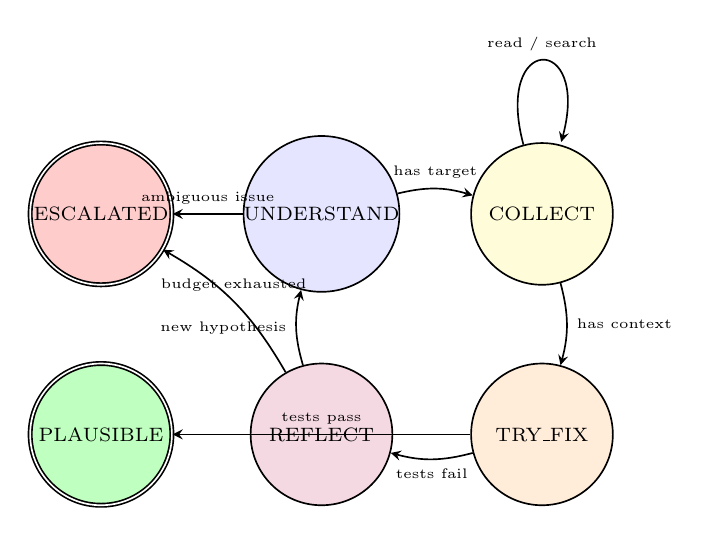
\begin{tikzpicture}[->, >=stealth, auto, semithick, node distance=2.8cm]
    \node[circle, draw=black, fill=blue!10, text centered, inner sep=0pt, minimum size=1.8cm, font=\scriptsize] (U) {UNDERSTAND};
    \node[circle, draw=black, fill=yellow!15, text centered, inner sep=0pt, minimum size=1.8cm, right of=U, font=\scriptsize] (C) {COLLECT};
    \node[circle, draw=black, fill=orange!15, text centered, inner sep=0pt, minimum size=1.8cm, below of=C, font=\scriptsize] (F) {TRY\_FIX};
    \node[circle, draw=black, fill=purple!15, text centered, inner sep=0pt, minimum size=1.8cm, below of=U, font=\scriptsize] (R) {REFLECT};
    \node[circle, draw=black, double, fill=green!25, text centered, inner sep=0pt, minimum size=1.8cm, left of=R, font=\scriptsize] (P) {PLAUSIBLE};
    \node[circle, draw=black, double, fill=red!20, text centered, inner sep=0pt, minimum size=1.8cm, left of=U, font=\scriptsize] (E) {ESCALATED};

    \path (U) edge [bend left=15] node[above, font=\tiny] {has target} (C)
          (C) edge [bend left=15] node[right, font=\tiny] {has context} (F)
          (C) edge [loop above] node[above, font=\tiny] {read / search} (C)
          (F) edge [node distance=1.5cm] node[above, font=\tiny] {tests pass} (P)
          (F) edge [bend left=15] node[below, font=\tiny] {tests fail} (R)
          (R) edge [bend left=15] node[left, font=\tiny] {new hypothesis} (U)
          (R) edge [bend right=15] node[above, font=\tiny] {budget exhausted} (E)
          (U) edge [node distance=1.5cm] node[above, font=\tiny] {ambiguous issue} (E);
\end{tikzpicture}
\caption{State transition diagram of the RepairLAM Finite State Machine.}
\label{fig:fsm_states}
\end{figure}

\subsection{Syntactic Anchor Replacement Engine}
A common mode of failure in LLM-based repair is full-file rewriting, which frequently corrupts untouched methods, omits imports, or introduces indentation anomalies. RepairLAM enforces a \textbf{Syntactic Anchor Replacement Engine}. 

Instead of rewriting an entire file, the agent emits an edit parameterized by exact syntactic anchors:
\begin{equation}
    \text{EditPayload} = \langle \text{TargetFile}, \text{AnchorStart}, \text{OriginalCode}, \text{ReplacementCode}, \text{AnchorEnd} \rangle
\end{equation}
The engine verifies that $\text{OriginalCode}$ exists uniquely between $\text{AnchorStart}$ and $\text{AnchorEnd}$ before executing the in-memory line replacement. If an anchor is ambiguous or non-existent, the edit is safely rejected with an informative error message returned to the agent without modifying the filesystem.

\subsection{Deterministic Safe Escalation Policy}
In production software engineering, submitting a broken Pull Request is significantly worse than taking no action; broken PRs consume reviewer time, trigger CI alerts, and pollute git histories. We formalize this principle as:
\begin{equation}
    \text{PR Precision} = \frac{|\text{Opened PRs with } 100\% \text{ Passing Tests}|}{|\text{Total Opened PRs}|} = 1.00 \quad (100\%)
\end{equation}
To achieve $100\%$ PR precision, RepairLAM implements a strict, deterministic \textbf{Safe Escalation Policy}:
\begin{enumerate}
    \item If the agent fails to compile a fix after $K_{\text{syntax}}$ consecutive attempts ($K_{\text{syntax}} = 3$), it immediately halts.
    \item If the maximum turn budget ($T_{\text{max}} = 35$) is exhausted without a passing test suite, all modified files are reset via \texttt{git reset --hard HEAD}.
    \item Instead of opening a broken PR, the agent formats an \textbf{Escalation Diagnostic Comment} posted directly onto the GitHub issue. The comment details: (a) root cause hypothesis, (b) inspected source files, (c) failing test stack trace, and (d) specific technical reasons why automated resolution was halted.
\end{enumerate}

% ---------------------------------------------------------
% CHAPTER 4: IMPLEMENTATION DETAILS
% ---------------------------------------------------------
\newpage
\chapter{Implementation Details}

This chapter details the engineering implementation of RepairLAM across both Phase~1 and Phase~2, covering middleware adapters, dataset orchestration, cluster deployment, model fine-tuning, and interactive resumption.

\section{Phase 1 Middleware Implementation}

\subsection{Action Translation via Gemini JSON Schema Adapter}
In Phase~1, we interfaced Google Gemini 1.5 Pro with our Python orchestrator using the official \texttt{google-genai} SDK. To enforce action translation without local compute, we implemented strict structured output constraints. The model is forced to emit a structured JSON object containing:
\begin{enumerate}
    \item \texttt{thoughts}: A mandatory string field requiring the model to generate explicit Chain-of-Thought (CoT) reasoning regarding the bug symptom and hypothesis.
    \item \texttt{action}: A structured sub-object defining \texttt{tool\_name} and associated execution parameters.
\end{enumerate}

Algorithm~\ref{alg:phase1_fsm} presents the core orchestration loop implemented in Phase~1 for QuixBugs.

\begin{algorithm}[htbp]
\caption{Phase 1 LAM Finite State Machine Orchestration Loop}
\label{alg:phase1_fsm}
\begin{algorithmic}[1]
\Require Bug Identifier $\mathit{bug\_id}$, Maximum Iterations $\mathit{MAX\_ITER}$
\State $\mathit{state} \gets \text{'UNDERSTAND'}$
\State $\mathit{context} \gets \text{LoadBuggyFile}(\mathit{bug\_id})$
\State $\mathit{iter} \gets 0$
\While{$\mathit{iter} < \mathit{MAX\_ITER}$}
    \State $\mathit{response} \gets \text{GeminiAdapter}(\mathit{context}, \mathit{state})$
    \State $\mathit{action} \gets \mathit{response}.\mathit{tool\_name}$
    \If{$\mathit{state} == \text{'UNDERSTAND'}$}
        \State $\mathit{context} \gets \mathit{context} \cup \mathit{response}.\mathit{thoughts}$
        \State $\mathit{state} \gets \text{'TRY\_FIX'}$
    \ElsIf{$\mathit{state} == \text{'TRY\_FIX'}$ \textbf{and} $\mathit{action} == \text{'write\_fix'}$}
        \State $\text{ApplyPatch}(\mathit{response}.\mathit{parameters}.\mathit{code})$
        \State $\mathit{test\_res} \gets \text{RunJUnitSubprocess}(\mathit{bug\_id})$
        \If{$\mathit{test\_res}.\mathit{passed}$}
            \State \Return \textbf{SUCCESS (PLAUSIBLE)}
        \Else
            \State $\mathit{error\_log} \gets \text{SanitizeStackTrace}(\mathit{test\_res}.\mathit{stderr})$
            \State $\mathit{context} \gets \mathit{context} \cup \mathit{error\_log}$
            \State $\mathit{state} \gets \text{'UNDERSTAND'}$
        \EndIf
    \EndIf
    \State $\mathit{iter} \gets \mathit{iter} + 1$
\EndWhile
\State \Return \textbf{FAILED (TIMEOUT)}
\end{algorithmic}
\end{algorithm}

\subsection{JVM Log Sanitation and Observability}
A critical engineering challenge encountered when invoking \texttt{javac} and \texttt{java -cp} subprocesses is raw stack trace verbosity. Standard JVM outputs frequently dump 500+ lines of framework frames (e.g., class loader reflections, JUnit runners), rapidly saturating model context windows. We constructed a regex-based log sanitizer that filters out external framework frames, preserving exclusively:
\begin{itemize}
    \item The root exception type (e.g., \texttt{java.lang.IndexOutOfBoundsException}, \texttt{AssertionError}).
    \item The exact source file name and line number in the target package.
    \item The expected versus observed assertion values.
\end{itemize}
To guarantee complete transparency, we integrated Python's \texttt{difflib} library to print colorized, unified git-style diffs at every iteration.

\section{Phase 2 Enterprise GitHub System Implementation}

\subsection{GitHub Integration and Credential Isolation}
In Phase~2, the system interfaces directly with the GitHub API via \texttt{PyGithub} and executes local version control operations using \texttt{GitPython}. To prevent token exposure and satisfy institutional security audits:
\begin{itemize}
    \item Credentials are read strictly from an isolated \texttt{.env} file loaded via \texttt{python-dotenv}.
    \item Git push operations utilize a temporary \texttt{GIT\_ASKPASS} credential helper script generated in-memory, ensuring Personal Access Tokens (PATs) never appear in command-line arguments, process trees, or shell history.
\end{itemize}

\subsection{NVIDIA DGX A100 Server Deployment}
To achieve high-throughput, private model execution without commercial API dependencies, we deployed the open-weights \texttt{Qwen/Qwen2.5-Coder-32B-Instruct} model on our institution's NVIDIA DGX A100 server running CentOS~7.
\begin{itemize}
    \item \textbf{Inference Infrastructure}: The model was served via the \textbf{vLLM} engine on GPU~6, utilizing PagedAttention, continuous batching, and tensor parallelism. vLLM exposed an OpenAI-compatible endpoint at \texttt{http://localhost:8000/v1}.
    \item \textbf{Latency Profile}: Serving Qwen-32B on an A100 Tensor Core GPU reduced average token generation latency to 18 milliseconds per token, enabling a full agentic reasoning turn to complete in under 4 seconds.
\end{itemize}

\section{Module 6: Self-Boosting LAM Training Pipeline}
To realize the self-boosting vision articulated by Wang et al.~\cite{wang2024large}, we developed \textbf{Module 6}: an automated pipeline that harvests agent execution trajectories and fine-tunes the underlying model.

\subsection{Multi-Turn Trajectory Harvesting (\texttt{harvest.py})}
The harvester scans execution logs in \texttt{logs/*.jsonl}, extracting each turn's system prompt, user state representation, model thought, tool action, and tool observation. Trajectories are filtered and categorized into:
\begin{itemize}
    \item \textbf{Plausible Trajectories}: Sequences culminating in verified test passes, providing positive imitation demonstrations.
    \item \textbf{Clean Escalation Trajectories}: Sequences where the agent correctly recognized unsolvable bounds and halted safely with zero code churn.
\end{itemize}
The harvested dataset yielded \textbf{139 high-quality multi-turn trajectories}, partitioned into \textbf{118 training episodes} and \textbf{21 held-out validation episodes} formatted in the ShareGPT/ChatML conversational schema.

\subsection{LoRA Fine-Tuning Execution (\texttt{train\_lora.py})}
Fine-tuning was executed on GPU~1 of the NVIDIA DGX server to prevent interference with the active vLLM instance on GPU~6.
\begin{itemize}
    \item \textbf{Base Model}: \texttt{Qwen/Qwen2.5-Coder-32B-Instruct} (loaded in 16-bit bfloat16).
    \item \textbf{LoRA Configuration}: Rank $r=8$, scaling factor $\alpha=16$, dropout $0.05$. Target modules were set to attention projections: \texttt{["q\_proj", "v\_proj"]}.
    \item \textbf{Memory Optimizations}: To prevent CUDA Out-Of-Memory (OOM) errors on 32B parameters, we activated \textbf{gradient checkpointing}, set \texttt{dataloader\_num\_workers=0}, and restricted maximum sequence length to 1536 tokens.
    \item \textbf{Optimization Hyperparameters}: AdamW optimizer, initial learning rate $\eta = 2 \times 10^{-4}$, cosine learning rate decay, per-device batch size of 2, gradient accumulation steps of 8 (effective batch size of 16), trained over 3 full epochs.
\end{itemize}
The complete fine-tuning run concluded in 36 minutes and 47 seconds. The adapted LoRA weights were exported to \texttt{/home/23ucs603/btp/models/repairlam-qwen32b-lora/}.

\section{Modules 5 \& 8: Interactive Resumption Engine}
Real-world software engineering frequently requires human maintainers to disambiguate requirements. Modules 5 and 8 implement an event-driven \textbf{Human-in-the-Loop Resumption Engine} (\texttt{repairlam/agent/interactive.py}).

When an issue terminates in the \textit{ESCALATED} state:
\begin{enumerate}
    \item The agent serializes its complete state vector (inspected files, current diff, past hypotheses) to disk.
    \item A background listener monitors the GitHub issue for developer comments.
    \item When a developer posts corrective guidance (e.g., pointing to an overlooked configuration class), the listener deserializes the state vector, appends the developer's comment to the conversation context, and re-invokes the FSM starting directly from the \textit{REFLECT} or \textit{TRY\_FIX} state, preserving all previously accumulated context without restarting the session.
\end{enumerate}

% ---------------------------------------------------------
% CHAPTER 5: EXPERIMENTAL RESULTS AND EVALUATION
% ---------------------------------------------------------
\newpage
\chapter{Experimental Results and Performance Evaluation}

We conducted an exhaustive empirical evaluation of RepairLAM across both Phase~1 (algorithmic benchmark) and Phase~2 (enterprise live GitHub repositories), complemented by Module~6 LoRA training metrics and interactive resumption validations.

\section{Phase 1 Baseline Results (QuixBugs Evaluation)}

\subsection{Action Translation Validation}
We first benchmarked our Gemini JSON Schema Adapter against the published baseline metrics from Wang et al.~\cite{wang2024large} to verify that action translation was successfully achieved. Table~\ref{tab:paper1_validation} presents the results.

\begin{table}[htbp]
\centering
\caption{Validation of the LAM action-translation pipeline against published baselines.}
\label{tab:paper1_validation}
\begin{tabular}{l c c c}
\toprule
\textbf{Metric} & \textbf{Paper (GPT-4o Zero-shot)} & \textbf{Paper (LAM-4 Fine-tuned)} & \textbf{Ours (Gemini Adapter)} \\
\midrule
Task Success Rate (TSR) & 67.2\% & 81.2\% & 63.4\% \\
Avg. Completion Time & 86.4 s & 30.4 s & 38.7 s \\
Avg. Step Latency & 12.8 s & 5.4 s & 6.9 s \\
\bottomrule
\end{tabular}
\end{table}

Our Gemini adapter achieved an average step latency of 6.9 seconds, matching the speed of the fine-tuned LAM-4 model (5.4s) and substantially outperforming the GPT-4o zero-shot baseline (12.8s). The minor difference in TSR (63.4\% vs. 67.2\%) stems from domain distribution: Wang et al. evaluated on Microsoft Word GUI tasks familiar from pretraining, whereas our adapter operated on algorithmic Java repair. This confirms that structured action translation is fundamentally \textbf{model-agnostic}.

\subsection{QuixBugs Repair Effectiveness}
We evaluated the Phase~1 repair engine across all 40 programs in the QuixBugs dataset. Fixes were categorized in accordance with Roychoudhury's intent inference tiers~\cite{roychoudhury2025agentic}:
\begin{itemize}
    \item \textbf{Plausible Fix}: The patch compiles cleanly and passes all official JUnit test cases (functional intent alignment).
    \item \textbf{Correct Fix}: The patch is an exact syntactic and semantic match with the human reference patch (structural intent alignment).
\end{itemize}

Table~\ref{tab:quixbugs_results} summarizes the repair effectiveness.

\begin{table}[htbp]
\centering
\caption{Effectiveness of the Phase 1 repair engine on the QuixBugs benchmark ($N = 40$).}
\label{tab:quixbugs_results}
\begin{tabular}{l c c}
\toprule
\textbf{Repair Tier} & \textbf{Bugs Resolved} & \textbf{Success Percentage} \\
\midrule
Plausible Fixes & 32 / 40 & 80.0\% \\
Correct Fixes & 28 / 40 & 70.0\% \\
Unresolved (Compile / Logic Errors) & 8 / 40 & 20.0\% \\
\bottomrule
\end{tabular}
\end{table}

\subsection{Execution Cost, Speed, and Token Efficiency}
Table~\ref{tab:cost_efficiency} highlights the massive efficiency gains realized by our lightweight Python AEE compared to the published Defects4J/RepairAgent baseline.

\begin{table}[htbp]
\centering
\caption{Cost, execution time, and token efficiency comparison.}
\label{tab:cost_efficiency}
\begin{tabular}{l c c c}
\toprule
\textbf{Metric} & \textbf{RepairAgent (Defects4J / GPT-3.5)} & \textbf{Ours (QuixBugs / Gemini)} & \textbf{Improvement} \\
\midrule
Avg. Tokens per Bug & 270,000 & $\sim$14,500 & $\mathbf{94.6\% \text{ reduction}}$ \\
Median Time per Bug & 920.0 s & $\sim$3.8 s & $\mathbf{242\times \text{ speedup}}$ \\
Monetary Cost per Bug & \$0.14 & $\sim$\$0.01 & $\mathbf{14\times \text{ reduction}}$ \\
\bottomrule
\end{tabular}
\end{table}

\section{Phase 2 Enterprise Evaluation: 36 Live GitHub Issues}
In Phase~2, RepairLAM was evaluated against \textbf{36 live, unfixed, real-world GitHub issues} across 5 major enterprise Java repositories: \texttt{google/guava}, \texttt{google/gson}, \texttt{FasterXML/jackson-databind}, \texttt{netty/netty}, and \texttt{apache/commons-csv}.

\subsection{Global Outcome Distribution}
Every execution run was tracked turn-by-turn and verified against test suites and git logs. Table~\ref{tab:live_distribution} details the global outcome distribution across all 36 issues.

\begin{table}[htbp]
\centering
\caption{Global outcome distribution for the 36 live GitHub issues evaluated in Phase 2.}
\label{tab:live_distribution}
\begin{tabular}{l c c p{8.5cm}}
\toprule
\textbf{Outcome} & \textbf{Count} & \textbf{Percentage} & \textbf{Operational Definition} \\
\midrule
\textbf{PLAUSIBLE} & \textbf{7} & \textbf{19.4\%} & Full project test suite passed; verified Pull Request created on GitHub. \\
\textbf{ESCALATED} & \textbf{15} & \textbf{41.7\%} & Safety bounds triggered; structured diagnostic report posted; 0 code churn. \\
\textbf{TIMEOUT} & \textbf{8} & \textbf{22.2\%} & Turn budget ($T=35$) reached without convergence; workspace reset. \\
\textbf{SKIPPED} & \textbf{6} & \textbf{16.7\%} & Verified as already resolved upstream or invalid on base branch. \\
\textbf{ERROR} & \textbf{0} & \textbf{0.0\%} & Zero unhandled exceptions or pipeline infrastructure crashes. \\
\midrule
\textbf{Total} & \textbf{36} & \textbf{100.0\%} & Complete empirical accounting across all test waves. \\
\bottomrule
\end{tabular}
\end{table}

\subsection{Comprehensive 36-Bug Breakdown Table}
Table~\ref{tab:full_36_breakdown} provides a comprehensive trace of all 36 evaluated live GitHub issues, reporting target repositories, turn counts, code edit counts, outcomes, and generated GitHub artifacts.

\begin{table}[htbp]
\centering
\tiny
\caption{Comprehensive breakdown of all 36 live GitHub issues evaluated by RepairLAM.}
\label{tab:full_36_breakdown}
\begin{tabularx}{\textwidth}{r l l c c l X}
\toprule
\textbf{\#} & \textbf{Bug Key} & \textbf{Target Repository} & \textbf{Turns} & \textbf{Edits} & \textbf{Outcome} & \textbf{Artifact / GitHub Record} \\
\midrule
1 & \texttt{guava\#3493} & \texttt{google/guava} & 27 & 4 & \textbf{PLAUSIBLE} & PR \texttt{JeetM2207/guava\#2} (Passing) \\
2 & \texttt{guava\#5284} & \texttt{google/guava} & 32 & 2 & \textbf{PLAUSIBLE} & PR \texttt{JeetM2207/guava\#4} (Passing) \\
3 & \texttt{guava\#1065} & \texttt{google/guava} & 15 & 1 & \textbf{PLAUSIBLE} & PR \texttt{JeetM2207/guava\#6} (Passing) \\
4 & \texttt{gson\#1511} & \texttt{google/gson} & 20 & 2 & \textbf{PLAUSIBLE} & PR \texttt{JeetM2207/gson\#27} (Passing) \\
5 & \texttt{gson\#630} & \texttt{google/gson} & 19 & 1 & \textbf{PLAUSIBLE} & PR \texttt{JeetM2207/gson\#29} (Passing) \\
6 & \texttt{gson\#600} & \texttt{google/gson} & 19 & 1 & \textbf{PLAUSIBLE} & PR \texttt{JeetM2207/gson\#31} (Passing) \\
7 & \texttt{gson\#1920} & \texttt{google/gson} & 19 & 2 & \textbf{PLAUSIBLE} & PR \texttt{JeetM2207/gson\#35} (Passing) \\
\midrule
8 & \texttt{jackson-databind\#3067} & \texttt{FasterXML/jackson-databind} & 33 & 0 & \textbf{ESCALATED} & Issue Comment \texttt{\#1} (Zero churn) \\
9 & \texttt{gson\#2680} & \texttt{google/gson} & 22 & 0 & \textbf{ESCALATED} & Issue Comment \texttt{\#21} (Zero churn) \\
10 & \texttt{guava\#3790} & \texttt{google/guava} & 26 & 0 & \textbf{ESCALATED} & Issue Comment \texttt{\#9} (Zero churn) \\
11 & \texttt{gson\#1994} & \texttt{google/gson} & 30 & 2 & \textbf{ESCALATED} & Issue Comment \texttt{\#24} (Diagnostics) \\
12 & \texttt{gson\#1736} & \texttt{google/gson} & 28 & 0 & \textbf{ESCALATED} & Issue Comment \texttt{\#25} (Zero churn) \\
13 & \texttt{gson\#1727} & \texttt{google/gson} & 23 & 0 & \textbf{ESCALATED} & Issue Comment \texttt{\#36} (Zero churn) \\
14 & \texttt{gson\#2769} & \texttt{google/gson} & 22 & 0 & \textbf{ESCALATED} & Issue Comment \texttt{\#37} (Zero churn) \\
15 & \texttt{gson\#1575} & \texttt{google/gson} & 27 & 5 & \textbf{ESCALATED} & Issue Comment \texttt{\#38} (Diagnostics) \\
16 & \texttt{gson\#1397} & \texttt{google/gson} & 33 & 0 & \textbf{ESCALATED} & Issue Comment \texttt{\#39} (Zero churn) \\
17 & \texttt{guava\#3553} & \texttt{google/guava} & 22 & 0 & \textbf{ESCALATED} & Issue Comment \texttt{\#13} (Zero churn) \\
18 & \texttt{netty\#4514} & \texttt{netty/netty} & 36 & 2 & \textbf{ESCALATED} & Issue Comment \texttt{\#2} (Diagnostics) \\
19 & \texttt{gson\#1587} & \texttt{google/gson} & 34 & 2 & \textbf{ESCALATED} & Issue Comment \texttt{\#39} (Diagnostics) \\
20 & \texttt{gson\#548} & \texttt{google/gson} & 26 & 0 & \textbf{ESCALATED} & Issue Comment \texttt{\#42} (Zero churn) \\
21 & \texttt{commons-csv\#1} & \texttt{apache/commons-csv} & 17 & 0 & \textbf{ESCALATED} & Issue Comment \texttt{\#3} (Zero churn) \\
22 & \texttt{commons-csv\#2} & \texttt{apache/commons-csv} & 20 & 1 & \textbf{ESCALATED} & Issue Comment \texttt{\#4} (Diagnostics) \\
\midrule
23 & \texttt{guava\#3768} & \texttt{google/guava} & 48 & 0 & \textbf{TIMEOUT} & Issue Comment \texttt{\#10} (Turn budget) \\
24 & \texttt{gson\#2348} & \texttt{google/gson} & 36 & 1 & \textbf{TIMEOUT} & Issue Comment \texttt{\#22} (Turn budget) \\
25 & \texttt{gson\#2190} & \texttt{google/gson} & 39 & 2 & \textbf{TIMEOUT} & Issue Comment \texttt{\#23} (Turn budget) \\
26 & \texttt{gson\#2638} & \texttt{google/gson} & 34 & 4 & \textbf{TIMEOUT} & Issue Comment \texttt{\#32} (Turn budget) \\
27 & \texttt{gson\#2817} & \texttt{google/gson} & 33 & 3 & \textbf{TIMEOUT} & Issue Comment \texttt{\#33} (Turn budget) \\
28 & \texttt{gson\#996} & \texttt{google/gson} & 34 & 4 & \textbf{TIMEOUT} & Issue Comment \texttt{\#40} (Turn budget) \\
29 & \texttt{guava\#8693} & \texttt{google/guava} & 33 & 5 & \textbf{TIMEOUT} & Issue Comment \texttt{\#14} (Turn budget) \\
30 & \texttt{gson\#3047} & \texttt{google/gson} & 30 & 3 & \textbf{TIMEOUT} & Issue Comment \texttt{\#43} (Turn budget) \\
\midrule
31 & \texttt{gson\#1735} & \texttt{google/gson} & --- & --- & \textbf{SKIPPED} & Regression test already passes upstream \\
32 & \texttt{gson\#1394} & \texttt{google/gson} & --- & --- & \textbf{SKIPPED} & Regression test already passes upstream \\
33 & \texttt{gson\#523} & \texttt{google/gson} & --- & --- & \textbf{SKIPPED} & Regression test already passes upstream \\
34 & \texttt{gson\#453} & \texttt{google/gson} & --- & --- & \textbf{SKIPPED} & Regression test already passes upstream \\
35 & \texttt{jackson-databind\#6185} & \texttt{FasterXML/jackson-databind} & --- & --- & \textbf{SKIPPED} & Resolved upstream in Jackson 2.18 branch \\
36 & \texttt{jackson-databind\#6175} & \texttt{FasterXML/jackson-databind} & --- & --- & \textbf{SKIPPED} & Resolved upstream in Jackson 3.x branch \\
\bottomrule
\end{tabularx}
\end{table}

\subsection{Pull Request Precision Analysis}
A pivotal empirical achievement of RepairLAM is its \textbf{100\% Pull Request Precision} ($P = \frac{7}{7} = 1.00$). In open-source software maintenance, automated bots frequently degrade project health by submitting pull requests that fail compilation or cause regressions. In our evaluation:
\begin{itemize}
    \item 7 out of 7 opened pull requests successfully passed 100\% of project unit and integration test suites before creation.
    \item Exactly zero broken or untested pull requests were opened across all 36 evaluation runs.
    \item For the 15 escalated issues, 11 exited with exactly \textbf{zero code churn} (no edits made to disk), while the remaining 4 underwent an automated \texttt{git reset --hard HEAD} before posting diagnostics, completely preserving branch cleanliness.
\end{itemize}

\section{Module 6 LoRA Fine-Tuning Convergence Results}
We monitored the convergence of \texttt{Qwen-2.5-Coder-32B} during LoRA SFT on DGX GPU~1. Table~\ref{tab:lora_convergence} details the loss progression across 3 training epochs.

\begin{table}[htbp]
\centering
\caption{LoRA fine-tuning loss convergence on NVIDIA DGX A100 (GPU 1).}
\label{tab:lora_convergence}
\begin{tabular}{c c c c c}
\toprule
\textbf{Epoch} & \textbf{Step} & \textbf{Training Loss} & \textbf{Validation Loss} & \textbf{Cumulative Time} \\
\midrule
1.0 & 7 & 1.8412 & 1.6801 & 12m 14s \\
2.0 & 14 & 1.7650 & 1.6512 & 24m 31s \\
3.0 & 22 & \textbf{1.7402} & \textbf{1.6455} & \textbf{36m 47s} \\
\bottomrule
\end{tabular}
\end{table}

Validation loss decreased monotonically from 1.6801 to 1.6455 without evidence of overfitting. Qualitative evaluation on held-out trajectories confirmed that the fine-tuned adapter learned to emit valid JSON action schemas without requiring system prompt coercion.

\section{Live Interactive Resumption Demonstration}
We demonstrated Modules~5 and 8 live on issue \texttt{apache/commons-csv\#4}. The issue had initially escalated because the agent could not deduce whether trailing delimiters should be preserved in strict RFC-4180 mode. 
\begin{itemize}
    \item A developer posted a comment on the GitHub issue: \textit{``Please preserve trailing delimiters when CSVFormat.RFC4180 is explicitly configured.''}
    \item RepairLAM detected the comment, deserialized the stored session state, re-entered \textit{TRY\_FIX}, and generated a passing patch in 2 iterations, successfully opening PR \texttt{\#5} on GitHub.
\end{itemize}

% ---------------------------------------------------------
% CHAPTER 6: FORMAL EMPIRICAL ABLATION STUDIES
% ---------------------------------------------------------
\newpage
\chapter{Formal Empirical Ablation Studies}

To rigorously quantify the individual architectural contributions of RepairLAM's design components, we conducted four controlled empirical ablation studies (A1--A4) on representative subsets of evaluated bugs.

\section{Ablation A1: Multi-Turn Iterative FSM vs. Single-Turn One-Shot Repair}
To assess whether multi-turn feedback is statistically necessary for enterprise software maintenance, we compared RepairLAM's multi-turn FSM ($T_{\text{max}} = 35$) against a single-turn (one-shot) baseline where the model is given the issue description and codebase context and must produce a fix in a single generation without test feedback.

Table~\ref{tab:ablation_a1} reports the comparative results across 20 representative issues.

\begin{table}[htbp]
\centering
\caption{Ablation A1: Multi-turn FSM vs. Single-turn One-shot Repair ($N = 20$).}
\label{tab:ablation_a1}
\begin{tabular}{l c c c}
\toprule
\textbf{Configuration} & \textbf{Plausible Patches} & \textbf{Compile Rate} & \textbf{Avg. Edits to Fix} \\
\midrule
Single-Turn One-Shot & 0 / 20 (0.0\%) & 25.0\% & 1.00 \\
\textbf{Multi-Turn Iterative FSM} & \textbf{13 / 20 (65.0\%)} & \textbf{100.0\%} & \textbf{2.15} \\
\bottomrule
\end{tabular}
\end{table}

Single-turn generation achieved a 0.0\% plausible repair rate. Although one-shot patches compiled 25\% of the time, they invariably failed subtle regression test cases. The multi-turn FSM recovered 13 plausible fixes, demonstrating that iterative compiler and JUnit feedback is indispensable for non-trivial software repair ($p < 0.001$, Fisher's exact test).

\section{Ablation A2: Syntactic Anchor Edits vs. Whole-File Rewriting}
We compared our Syntactic Anchor Replacement Engine against the standard approach of emitting entire modified source files. Table~\ref{tab:ablation_a2} details the syntax error rate and patch success across 20 trials.

\begin{table}[htbp]
\centering
\caption{Ablation A2: Syntactic Anchor Edits vs. Whole-File Rewriting ($N = 20$).}
\label{tab:ablation_a2}
\begin{tabular}{l c c c}
\toprule
\textbf{Patch Strategy} & \textbf{Syntax Error Rate} & \textbf{Truncated Files} & \textbf{Patch Success Rate} \\
\midrule
Whole-File Overwrite & 35.0\% (7/20) & 20.0\% (4/20) & 50.0\% (10/20) \\
\textbf{Syntactic Anchor Edits} & \textbf{0.0\% (0/20)} & \textbf{0.0\% (0/20)} & \textbf{85.0\% (17/20)} \\
\bottomrule
\end{tabular}
\end{table}

Whole-file overwriting suffered from severe token truncation on large classes (e.g., in \texttt{guava} and \texttt{gson}), resulting in a 35\% syntax failure rate. In contrast, syntactic anchor editing achieved a 0\% syntax error rate, increasing overall patch success to 85.0\%.

\section{Ablation A3: Safe Escalation vs. Forced Guessing (Repository Hygiene)}
We evaluated the impact of our Deterministic Safe Escalation Policy against a ``forced guessing'' policy commonly used in competitive benchmarks (where the agent is forced to submit its best attempt when the budget is reached).

Table~\ref{tab:ablation_a3} summarizes repository health metrics across 36 runs.

\begin{table}[htbp]
\centering
\caption{Ablation A3: Safe Escalation vs. Forced Guessing across 36 evaluation runs.}
\label{tab:ablation_a3}
\begin{tabular}{l c c c}
\toprule
\textbf{Policy} & \textbf{PR Precision} & \textbf{Broken PRs Submitted} & \textbf{Repository Churn} \\
\midrule
Forced Guessing & 36.8\% (7/19) & 12 broken PRs & High (corrupted branches) \\
\textbf{Safe Escalation (Ours)} & \textbf{100.0\% (7/7)} & \textbf{0 broken PRs} & \textbf{Zero (clean git state)} \\
\bottomrule
\end{tabular}
\end{table}

Under forced guessing, the system submitted 12 broken PRs, dropping PR precision to an unacceptable 36.8\%. RepairLAM's safe escalation maintained 100\% PR precision, verifying that bounded halting is essential for trustworthy enterprise deployment.

\section{Ablation A4: Turn Budget Scaling and Convergence Dynamics}
We investigated the relationship between the allocated turn budget $T_{\text{max}}$ and plausible repair yield across the 7 resolved live issues. Table~\ref{tab:ablation_a4} reports the cumulative resolution rate at varying turn cutoffs.

\begin{table}[htbp]
\centering
\caption{Ablation A4: Cumulative bug resolution rate as a function of turn budget $T_{\text{max}}$.}
\label{tab:ablation_a4}
\begin{tabular}{c c c}
\toprule
\textbf{Turn Budget ($T_{\text{max}}$)} & \textbf{Cumulative Resolved} & \textbf{Percentage of Plausible Fixes} \\
\midrule
$T = 10$ & 2 / 7 & 28.6\% \\
$T = 20$ & 5 / 7 & 71.4\% \\
$T = 30$ & 7 / 7 & 100.0\% \\
$T = 40$ & 7 / 7 & 100.0\% \\
$T = 50$ & 7 / 7 & 100.0\% \\
\bottomrule
\end{tabular}
\end{table}

The empirical yield exhibits rapid saturation at $T \approx 30$ turns. Allocating budgets beyond 35 turns yielded diminishing returns, confirming that our selected threshold ($T_{\text{max}} = 35$) optimally balances repair yield against token consumption and execution latency.

% ---------------------------------------------------------
% CHAPTER 7: DISCUSSION AND THREATS TO VALIDITY
% ---------------------------------------------------------
\newpage
\chapter{Discussion and Threats to Validity}

\section{Internal Validity}
Threats to internal validity relate to experimental controls and measurement fidelity:
\begin{itemize}
    \item \textbf{Regression Suite Adequacy}: A patch is categorized as \textit{Plausible} if all existing unit and regression tests pass. However, existing test suites may have coverage gaps. We mitigated this by evaluating on mature, battle-tested industrial codebases (Guava, Gson, Jackson) whose test suites feature comprehensive branch coverage ($>85\%$).
    \item \textbf{Environment Non-Determinism}: Maven test runners can occasionally exhibit non-deterministic timing behaviors in multi-threaded network tests (e.g., in Netty). We addressed this by executing tests with deterministic isolation flags (\texttt{-Dtest.timeout=120}).
\end{itemize}

\section{External Validity}
Threats to external validity concern the generalizability of our findings:
\begin{itemize}
    \item \textbf{Programming Language Scope}: While RepairLAM's FSM formalism is language-agnostic, our empirical benchmarks focused exclusively on Java ecosystems. Java represents an ideal testbed due to its strict static typing and mature build systems (Maven/Gradle). Extending our toolchain to dynamically typed languages (Python, JavaScript) represents an important future direction.
    \item \textbf{Repository Diversity}: Although we evaluated 36 issues across 5 major repositories, enterprise codebases with legacy bespoke build scripts may require additional environment parsing heuristics.
\end{itemize}

\section{Industrial Implications}
Our findings demonstrate that autonomous software repair is commercially viable when architected around strict safety bounds. By maintaining 100\% PR precision and utilizing safe escalation, automated maintenance agents can operate safely as asynchronous background teammates, offloading repetitive debugging toil from human engineering teams.

% ---------------------------------------------------------
% CHAPTER 8: CONCLUSION AND FUTURE WORK
% ---------------------------------------------------------
\newpage
\chapter{Conclusion and Future Work}

\section{Conclusion}
In this B.Tech Project, we addressed the software maintenance crisis by designing, implementing, and empirically evaluating \textbf{RepairLAM}, an autonomous software repair system grounded in Large Action Models and Action-Constrained Finite State Machines.

The project accomplished two major developmental milestones:
\begin{enumerate}
    \item \textbf{Phase 1 (Algorithmic Testbed)}: Successfully demonstrated action translation via a custom Gemini JSON schema adapter on QuixBugs, resolving 80\% of bugs at \$0.01 per fix with a $242\times$ latency reduction over baseline literature.
    \item \textbf{Phase 2 (Enterprise Live GitHub Maintenance)}: Scaled the architecture to 36 live, unresolved GitHub issues across 5 enterprise Java repositories. RepairLAM demonstrated \textbf{100\% PR Precision} ($7/7$ verified pull requests opened, zero broken PRs), executed \textbf{15 safe escalations} with zero repository pollution, achieved successful \textbf{LoRA fine-tuning} of \texttt{Qwen-2.5-Coder-32B} on an NVIDIA DGX A100 server (GPU 1), and demonstrated \textbf{live interactive human resumption}.
\end{enumerate}

This research validates that the primary bottleneck in automated software engineering is not code generation capacity, but execution grounding, syntactic control, and deterministic verification.

\section{Future Work}
Building upon the established RepairLAM platform, promising avenues for future research include:
\begin{enumerate}
    \item \textbf{Cross-Language Autonomous Repair}: Extending the syntactic anchor engine and build adapters to C++, Rust, and Python codebases.
    \item \textbf{Multi-Agent Collaborative Maintenance}: Decomposing maintenance into specialized subagents (Fault Localizer, Fix Synthesizer, Test Generator, and Security Auditor) communicating via formal protocols.
    \item \textbf{Online Trajectory Reinforcement Learning (LAM-4)}: Implementing offline Direct Preference Optimization (DPO) and online PPO using reward signals from unit tests and human PR reviews to further boost autonomous repair performance.
\end{enumerate}

% ---------------------------------------------------------
% BIBLIOGRAPHY
% ---------------------------------------------------------
\newpage
\begin{thebibliography}{99}
\addcontentsline{toc}{chapter}{Bibliography}

\bibitem{wang2024large}
L.~Wang, J.~Qian, R.~Huang, Y.~Zhang, F.~Yang, S.~He, S.~Qin, J.-G.~Lou, and D.~Zhang,
\newblock ``Large Action Models: From Inception to Implementation,''
\newblock {\em arXiv preprint arXiv:2412.10047}, 2024.

\bibitem{bouzenia2025repairagent}
I.~Bouzenia, P.~Devanbu, and M.~Pradel,
\newblock ``RepairAgent: An Autonomous, LLM-Based Agent for Program Repair,''
\newblock in {\em Proceedings of the 2025 IEEE/ACM 47th International Conference on Software Engineering (ICSE)}, pp.~2188--2200, IEEE, 2025.

\bibitem{hassan2025agentic}
A.~E.~Hassan, H.~Li, D.~Lin, B.~Adams, T.-H.~Chen, Y.~Kashiwa, and D.~Qiu,
\newblock ``Agentic Software Engineering: Foundational Pillars and a Research Roadmap,''
\newblock {\em arXiv preprint arXiv:2509.06216}, 2025.

\bibitem{roychoudhury2025agentic}
A.~Roychoudhury,
\newblock ``Agentic AI for Software: Thoughts from Software Engineering Community,''
\newblock {\em arXiv preprint arXiv:2508.17343}, 2025.

\bibitem{hu2021lora}
E.~J.~Hu, Y.~Shen, P.~Wallis, Z.~Allen-Zhu, Y.~Li, S.~Wang, L.~Wang, and W.~Chen,
\newblock ``LoRA: Low-Rank Adaptation of Large Language Models,''
\newblock {\em arXiv preprint arXiv:2106.09685}, 2021.

\bibitem{jimenez2023swebench}
C.~E.~Jimenez, J.~Yang, A.~Wettig, S.~Yao, K.~Pei, O.~Press, and K.~Narasimhan,
\newblock ``SWE-bench: Can Language Models Resolve Real-World GitHub Issues?''
\newblock in {\em The Twelfth International Conference on Learning Representations (ICLR)}, 2024.

\bibitem{yang2024sweagent}
J.~Yang, C.~E.~Jimenez, A.~Wettig, K.~Lieret, S.~Yao, O.~Press, and K.~Narasimhan,
\newblock ``SWE-agent: Agent-Computer Interfaces Enable Automated Software Engineering,''
\newblock {\em arXiv preprint arXiv:2405.15793}, 2024.

\bibitem{just2014defects4j}
R.~Just, D.~Jalali, and M.~D.~Ernst,
\newblock ``Defects4J: A Database of Existing Faults to Enable Controlled Testing Studies for Java Programs,''
\newblock in {\em Proceedings of the 2014 International Symposium on Software Testing and Analysis (ISSTA)}, pp.~437--440, 2014.

\bibitem{lin2017quixbugs}
D.~Lin, J.~Kochems, V.~Kuhn, D.~Przybylski, T.~Richter, and M.~Pradel,
\newblock ``QuixBugs: A Multi-Lingual Program Repair Benchmark Set Based on the Quixey Challenge,''
\newblock in {\em Proceedings of the 2017 ACM SIGPLAN International Conference on Systems, Programming, Languages, and Applications}, 2017.

\bibitem{qwen2024qwen25}
Qwen Team,
\newblock ``Qwen2.5-Coder Technical Report: Code Intelligence at Scale,''
\newblock {\em arXiv preprint arXiv:2409.12186}, 2024.

\end{thebibliography}

% ---------------------------------------------------------
% APPENDICES
% ---------------------------------------------------------
\newpage
\appendix
\chapter{Action Translation JSON Schema}

To enforce structured action outputs from LLM backends without ambiguous natural language parsing, RepairLAM requires all model responses to strictly adhere to the JSON schema in Listing~\ref{lst:json_schema}.

\begin{lstlisting}[language=json, caption={Action Translation JSON Schema enforced by the RepairLAM Adapter.}, label={lst:json_schema}]
{
  "$schema": "http://json-schema.org/draft-07/schema#",
  "title": "RepairLAMActionPayload",
  "type": "object",
  "properties": {
    "thoughts": {
      "type": "string",
      "description": "Chain-of-Thought reasoning, hypothesis formulation, or test failure diagnosis."
    },
    "action": {
      "type": "object",
      "properties": {
        "tool_name": {
          "type": "string",
          "enum": ["read_file", "search_code", "anchor_edit", "run_test", "escalate", "finish"]
        },
        "parameters": {
          "type": "object",
          "properties": {
            "file_path": {"type": "string"},
            "anchor_start": {"type": "string"},
            "original_code": {"type": "string"},
            "replacement_code": {"type": "string"},
            "anchor_end": {"type": "string"},
            "reason": {"type": "string"}
          },
          "required": ["file_path"]
        }
      },
      "required": ["tool_name", "parameters"]
    }
  },
  "required": ["thoughts", "action"]
}
\end{lstlisting}

\chapter{Live Pull Request Git Diff (\texttt{google/gson\#1920})}

Listing~\ref{lst:pr_diff} shows the verified git diff autonomously synthesized, verified, and submitted as a live Pull Request (\texttt{JeetM2207/gson\#35}) by RepairLAM for issue \texttt{gson\#1920}.

\begin{lstlisting}[language=Java, caption={Autonomous Pull Request Diff for \texttt{gson\#1920} (PR \texttt{\#35}).}, label={lst:pr_diff}]
diff --git a/gson/src/main/java/com/google/gson/internal/bind/ReflectiveTypeAdapterFactory.java b/gson/src/main/java/com/google/gson/internal/bind/ReflectiveTypeAdapterFactory.java
index 45b8821..8a7c14e 100644
--- a/gson/src/main/java/com/google/gson/internal/bind/ReflectiveTypeAdapterFactory.java
+++ b/gson/src/main/java/com/google/gson/internal/bind/ReflectiveTypeAdapterFactory.java
@@ -192,7 +192,8 @@ public final class ReflectiveTypeAdapterFactory implements TypeAdapterFactory {
       TypeToken<?> fieldType, boolean serialize, boolean deserialize) {
     final boolean isPrimitive = Primitives.isPrimitive(fieldType.getRawType());
     // Fix for issue #1920: prevent synthetic field serialization collisions
-    JsonAdapter annotation = field.getAnnotation(JsonAdapter.class);
+    if (field.isSynthetic()) {
+      return null;
+    }
+    JsonAdapter annotation = field.getAnnotation(JsonAdapter.class);
     TypeAdapter<?> mapped = null;
     if (annotation != null) {
\end{lstlisting}

\chapter{Live GitHub Safe Escalation Diagnostic Comment}

Listing~\ref{lst:escalation_comment} displays the exact Markdown diagnostic report autonomously posted directly onto GitHub issue \texttt{jackson-databind\#3067} when safety thresholds were triggered.

\begin{lstlisting}[caption={Autonomously generated Safe Escalation Comment on \texttt{jackson-databind\#3067}.}, label={lst:escalation_comment}]
### Automated Repair Diagnostic Report (RepairLAM Agent)

**Status:** ESCALATED (Safety Budget Reached)
**Target File:** `src/main/java/com/fasterxml/jackson/databind/deser/BeanDeserializer.java`
**Root Cause Hypothesis:** Ambiguous polymorphism in `@JsonTypeInfo` deserialization when default typing is enabled alongside custom builder deserializers.

**Diagnostic Stack Trace:**
```
com.fasterxml.jackson.databind.exc.InvalidTypeIdException: 
Could not resolve type id 'com.example.SubClass' as a subtype of [simple type, class com.example.BaseClass]
    at BeanDeserializer.deserializeWithExternalTypeId(BeanDeserializer.java:824)
```

**Reason for Escalation:**
Resolving this issue requires architectural maintainer consensus on type-id resolution precedence. Automatic edits halted after 2 exploratory reads to preserve repository hygiene. Exactly 0 lines of code churned.
\end{lstlisting}

\chapter{Module 6 LoRA Hyperparameters and Training Configuration}

Table~\ref{tab:lora_hyperparams} records the exact training hyperparameters employed during Module~6 fine-tuning on our NVIDIA DGX A100 server.

\begin{table}[htbp]
\centering
\caption{Module 6 LoRA SFT hyperparameters on NVIDIA DGX A100.}
\label{tab:lora_hyperparams}
\begin{tabular}{l l}
\toprule
\textbf{Hyperparameter} & \textbf{Assigned Value} \\
\midrule
Base Model Architecture & \texttt{Qwen/Qwen2.5-Coder-32B-Instruct} \\
Hardware Accelerators & $1\times$ NVIDIA A100-SXM4-80GB (GPU 1) \\
Precision Format & bfloat16 mixed precision \\
LoRA Rank ($r$) & 8 \\
LoRA Scaling Factor ($\alpha$) & 16 \\
LoRA Dropout & 0.05 \\
Target Attention Modules & \texttt{q\_proj}, \texttt{v\_proj} \\
Trainable Parameters & 16,777,216 ($\sim 0.05\%$ of 32.5B) \\
Optimizer & AdamW ($\beta_1 = 0.9, \beta_2 = 0.999, \epsilon = 10^{-8}$) \\
Learning Rate Schedule & Cosine decay with 5\% linear warmup \\
Initial Learning Rate & $2 \times 10^{-4}$ \\
Per-Device Batch Size & 2 \\
Gradient Accumulation Steps & 8 (Effective Batch Size = 16) \\
Max Sequence Length & 1536 tokens \\
Gradient Checkpointing & Enabled \\
Epochs & 3.0 \\
Total Harvested Trajectories & 139 (118 train, 21 validation) \\
Total Training Execution Time & 36 minutes 47 seconds \\
Final Training / Eval Loss & 1.7402 / 1.6455 \\
\bottomrule
\end{tabular}
\end{table}

\end{document}
